%
% $RCSfile$
%
% Copyright (c) 2005-2006. Christian Heller. All rights reserved.
%
% Permission is granted to copy, distribute and/or modify this document
% under the terms of the GNU Free Documentation License, Version 1.1 or
% any later version published by the Free Software Foundation; with no
% Invariant Sections, with no Front-Cover Texts and with no Back-Cover
% Texts. A copy of the license is included in the section entitled
% "GNU Free Documentation License".
%
% http://www.cybop.net
% - Cybernetics Oriented Programming -
%
% http://www.resmedicinae.org
% - Information in Medicine -
%
% Version: $Revision$ $Date$ $Author$
% Authors: Christian Heller <christian.heller@tuxtax.de>
%

\subsection{Statics and Dynamics}
\label{statics_and_dynamics_heading}

Of the many scientific fields that have been touched and delivered design
ideas for CYBOP, only few can be elaborated in this article, due to the limited
space.

%
% $RCSfile$
%
% Copyright (c) 2002-2006. Christian Heller. All rights reserved.
%
% Permission is granted to copy, distribute and/or modify this document
% under the terms of the GNU Free Documentation License, Version 1.1 or
% any later version published by the Free Software Foundation; with no
% Invariant Sections, with no Front-Cover Texts and with no Back-Cover
% Texts. A copy of the license is included in the section entitled
% "GNU Free Documentation License".
%
% http://www.cybop.net
% - Cybernetics Oriented Programming -
%
% http://www.resmedicinae.org
% - Information in Medicine -
%
% Version: $Revision$ $Date$ $Author$
% Authors: Christian Heller <christian.heller@tuxtax.de>
%

\subsubsection{Code Reduction}
\label{code_reduction_heading}

In his book \emph{Programming Pearls} \cite[page 128]{bentley}, Jon Bentley
demonstrates \emph{Code Reduction} on the following graphics program example:

\begin{scriptsize}
    \begin{verbatim}
� � for i = [17, 43] set(i, 68)
� � for i = [18, 42] set(i, 69)
� � for j = [81, 91] set(30, j)
� � for j = [82, 92] set(31, j)
    \end{verbatim}
\end{scriptsize}

He suggests to replace the \emph{set} procedures that switch a
\emph{Picture Element} (Pixel) with suitable functions for drawing horizontal
and vertical lines:

\begin{scriptsize}
    \begin{verbatim}
� � hor(17, 43, 68)
� � hor(18, 42, 69)
� � vert(81, 91, 30)
� � vert(82, 92, 31)
    \end{verbatim}
\end{scriptsize}

This code, finally, gets reduced to pure data stored in an array:

\begin{scriptsize}
    \begin{verbatim}
� � h 17 43 68
� � h 18 42 69
� � v 81 91 30
� � v 82 92 31
    \end{verbatim}
\end{scriptsize}

The data can be read by an interpreter program which knows about their meaning.

Bentley's example shows in a nice way how knowledge can be extracted from program
source code. The graphic application's actual data are represented by the values
in the array above. All other functionality accessing and manipulating Pixels
directly does belong to system control and remains in the interpreter program.
Section \ref{cyboi_heading} will introduce an interpreter that is able to read
and handle \emph{general} knowledge, only on a much larger scale.

%
% $RCSfile: base_and_meta_level.tex,v $
%
% Copyright (C) 2002-2008. Christian Heller.
%
% Permission is granted to copy, distribute and/or modify this document
% under the terms of the GNU Free Documentation License, Version 1.1 or
% any later version published by the Free Software Foundation; with no
% Invariant Sections, with no Front-Cover Texts and with no Back-Cover
% Texts. A copy of the license is included in the section entitled
% "GNU Free Documentation License".
%
% http://www.cybop.net
% - Cybernetics Oriented Programming -
%
% http://www.resmedicinae.org
% - Information in Medicine -
%
% Version: $Revision: 1.1 $ $Date: 2008-08-19 20:41:05 $ $Author: christian $
% Authors: Christian Heller <christian.heller@tuxtax.de>
%

\subsection{Base- and Meta Level}
\label{base_and_meta_level_heading}
\index{Base Level}
\index{Meta Level}
\index{Reflective Technique}
\index{System- and Application Functionality}
\index{Bidirectional Dependency}

Reflective techniques as described in section \ref{reflection_heading} make use
of one so-called \emph{Base Level} and one or more \emph{Meta Levels}. The
reason for splitting a system's architecture in this way is the hope to be able
to move rather general \emph{System Functionality} into a meta level, while
leaving domain-specific \emph{Application Functionality} in the base level.
(Well, in his book \emph{Analysis Patterns -- Reusable Object Models}
\cite{fowler1997}, Fowler used meta levels to model general classes containing
not exclusively system- but also domain-specific functionality.) The conflicts
a design decision of that kind can bring with were described in section
\ref{broken_type_system_heading}, which -- above all -- criticised the
bidirectional dependencies.

However, what the proposition of reflective software patterns shows, is the
existence of a wish among software developers, to separate general system- from
more specific application functionality. And, as was shown in section
\ref{virtual_and_real_world_heading}, nature does exactly that. Yet while
reflective mechanisms use the same implementation techniques for system- as
well as for application-specific functionality, nature always treats passive
knowledge strictly separate from active system control (section
\ref{virtual_and_real_world_heading}). Bidirectional dependencies do not exist
between the both.

%
% $RCSfile$
%
% Copyright (c) 2005-2006. Christian Heller. All rights reserved.
%
% Permission is granted to copy, distribute and/or modify this document
% under the terms of the GNU Free Documentation License, Version 1.1 or
% any later version published by the Free Software Foundation; with no
% Invariant Sections, with no Front-Cover Texts and with no Back-Cover
% Texts. A copy of the license is included in the section entitled
% "GNU Free Documentation License".
%
% http://www.cybop.net
% - Cybernetics Oriented Programming -
%
% http://www.resmedicinae.org
% - Information in Medicine -
%
% Version: $Revision$ $Date$ $Author$
% Authors: Christian Heller <christian.heller@tuxtax.de>
%

\subsubsection{Application and Domain}
\label{application_and_domain_heading}

Over the years, it has turned out to be helpful in software design, to separate
\emph{Domain Knowledge} from \emph{Application Functionality}. In
one-or-another form, the architectural software patterns \cite{heller2005}
\emph{Layers}, \emph{Domain Model} and \emph{Model View Controller} (MVC) all
suggest to apply this principle.

The \emph{Tools \& Materials} approach \cite{tandm} talks of \emph{active}
applications (tools) working on \emph{passive} domain data (material). And also
\emph{System Family Engineering} \cite{domainengg} bases on a separate
treatment of domain and application, in form of \emph{Domain Engineering} (DE)
and \emph{Application Engineering} (AE).

An often neglected fact of these approaches is that not only the domain, but
also the application contains important business knowledge (figure
\ref{separation_figure}). The \emph{User Interface} (UI), for example, is
tailored for a specific business domain. And the logic behind, if not
contained in the UI itself, is often put in a \emph{Controller} which belongs
to the application$-$, not the domain layer.

\begin{figure}[ht]
    \begin{center}
        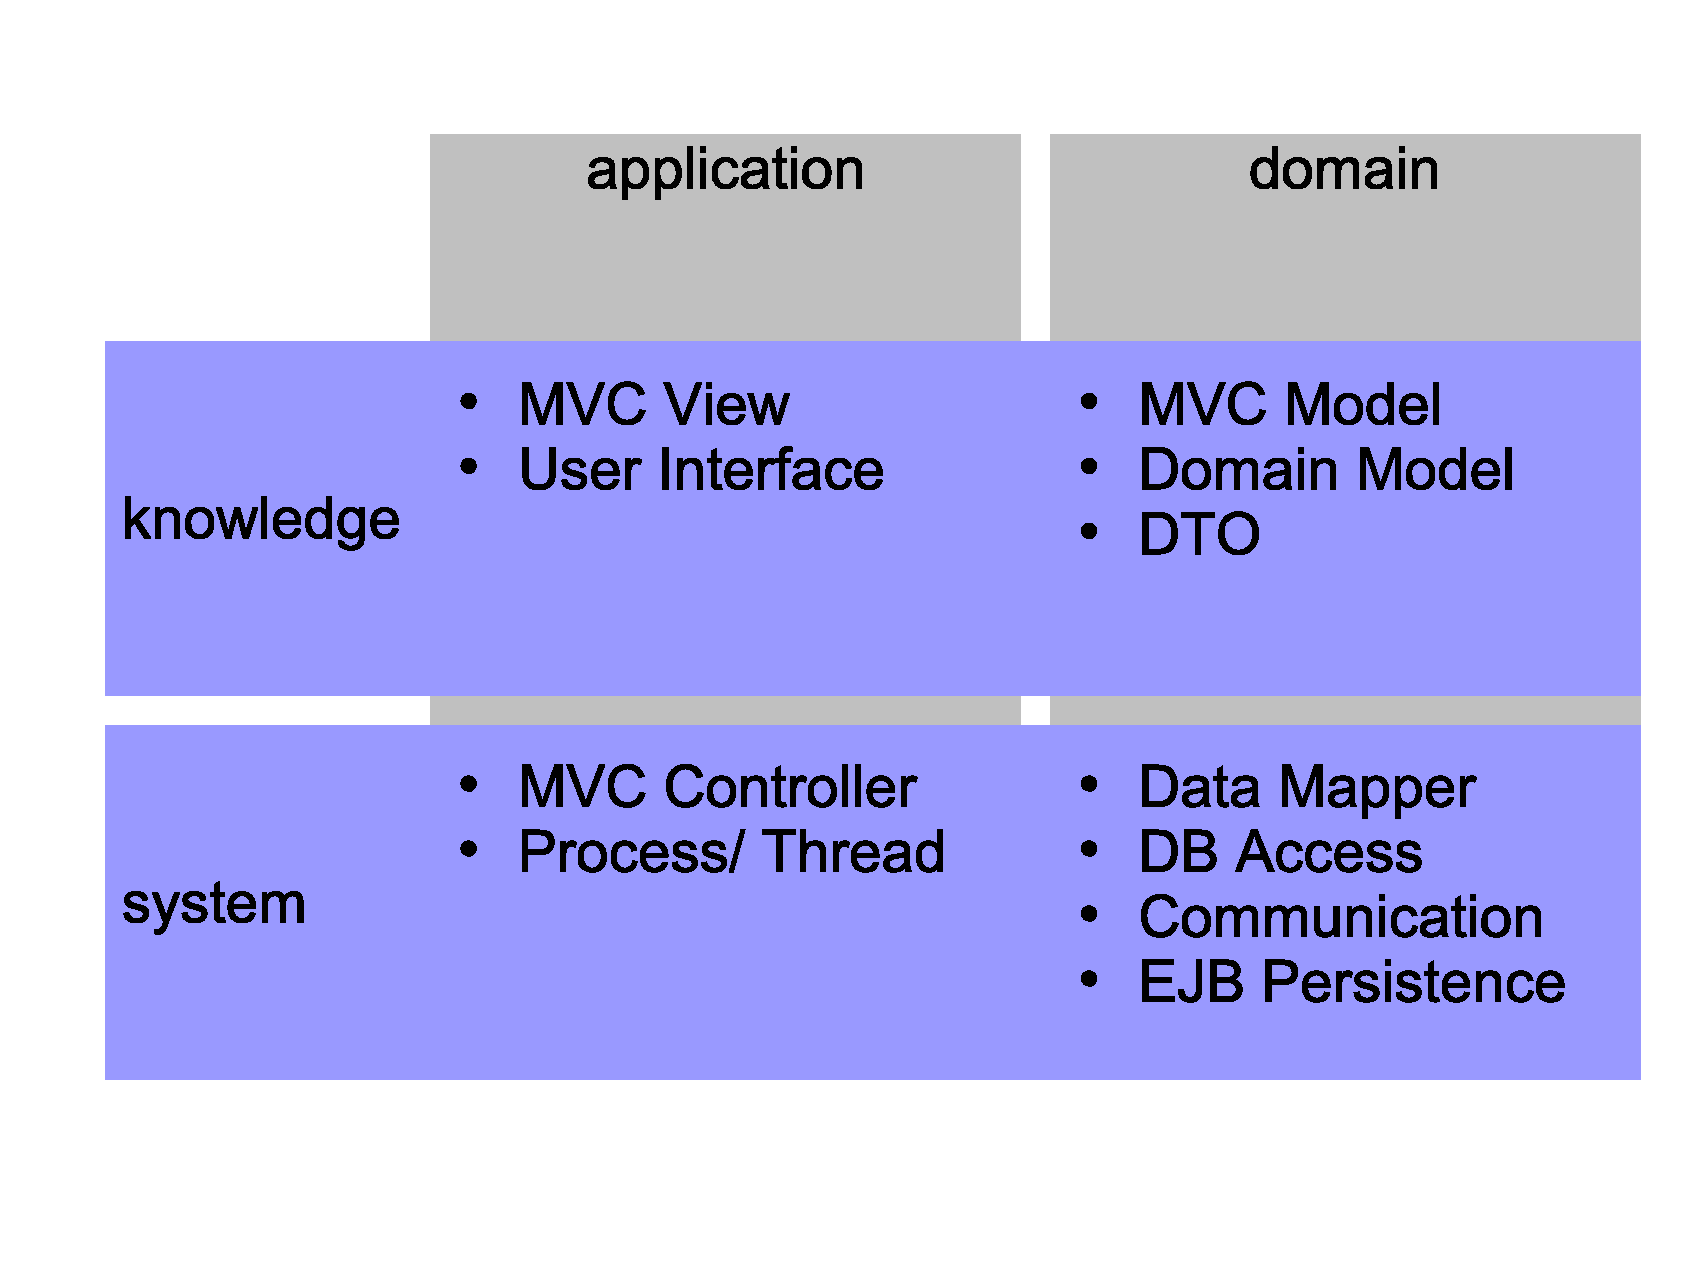
\includegraphics[scale=0.2]{vector/separation.eps}
        \caption{Different Knowledge Separations}
        \label{separation_figure}
    \end{center}
\end{figure}

Similarly, the domain often contains functionality which actually does belong
into the application process: \emph{Database} (DB) access is handled by help of
patterns like the \emph{Data Mapper} \cite{heller2005}, in which the mapper\\
objects contain \emph{Structured Query Language} (SQL) code to connect to a
\emph{Database Management System} (DBMS); \emph{Enterprise Java Beans} (EJB),
which should better be pure domain objects, imitate a \emph{Middleware}
providing persistence- or communication mechanisms, which originally have
nothing to do with the business knowledge they contain.

It is precisely this \emph{Mixup} of responsibilities between an application
system and its domain knowledge, that leads to multiple inter-dependencies and
hence unflexibility within a system. Instead, a separation should be made
between active \emph{System Control} and passive \emph{Knowledge}. A UI's
appearance would then be treated as domain knowledge, just as the logic of the
functions called through it. A data mapper would be transformed into a simple
\emph{Translator} -- similar to a \emph{Data Transfer Object} (DTO)
\cite{heller2005} -- that knows how to convert data from one domain model into
another; its DBMS access functionality, however, would be extracted and put
into the application system. Monstrosities like EJBs would likewise be opened
up and parted into their actual domain knowledge, and all other mechanisms
around -- the latter being moved into the application system.

To sum up this thought: The essential realisation here is that hardware-close
mechanisms like the ones necessary for data input/ output (i/o), enabling
inter-system communication, should be handled in an active application system
layer which was started as process on a computer, and \emph{not} be merged with
pure, passive domain knowledge. User interfaces and application logic which are
traditionally held in controller objects of the application layer, as well as
further business data models, should rather belong to a high-level knowledge
layer.

%
% $RCSfile$
%
% Copyright (c) 2002-2006. Christian Heller. All rights reserved.
%
% Permission is granted to copy, distribute and/or modify this document
% under the terms of the GNU Free Documentation License, Version 1.1 or
% any later version published by the Free Software Foundation; with no
% Invariant Sections, with no Front-Cover Texts and with no Back-Cover
% Texts. A copy of the license is included in the section entitled
% "GNU Free Documentation License".
%
% http://www.cybop.net
% - Cybernetics Oriented Programming -
%
% http://www.resmedicinae.org
% - Information in Medicine -
%
% Version: $Revision$ $Date$ $Author$
% Authors: Christian Heller <christian.heller@tuxtax.de>
%

\subsubsection{Platform Specific and -Independent}
\label{platform_specific_and_independent_heading}

The \emph{Model Driven Architecture} (MDA) \cite{mda} took a first step into
the right direction, by distinguishing \emph{Platform Independent Models}
(PIM), that is domain- and application logic, and \emph{Platform Specific Models}
(PSM), that is implementation technology. It encourages the use of automated
tools for defining and transforming these models.

While the definition, organisation and management of architectures (PIM) mostly
happen in the analysis- and design phase of a \emph{Software Engineering Process}
(SEP) (section \ref{abstraction_gaps_heading}), the generation of source code
(PSM) can be assigned to the implementation phase. The approach still has
weaknesses, and tools which can truly generate running systems are rare or not
existent, at least to what concerns more complex software systems -- not to
talk of the so-called \emph{Roundtrip Engineering}, which is managed by even
less tools.

Nevertheless, the trend clearly goes towards more model-centric approaches. The
aim of this work was to supply domain experts and application developers with a
\emph{Model Only} technology, allowing to create application systems that do
\emph{not} have to be transformed into classical implementation code any longer,
whereby the SEP abstraction gap number \emph{2} (figure \ref{gaps_figure})
could be closed conclusively. The knowledge schema introduced in section
\ref{knowledge_schema_heading} is a necessary prerequisite therefor.

%
% $RCSfile$
%
% Copyright (c) 2005-2006. Christian Heller. All rights reserved.
%
% Permission is granted to copy, distribute and/or modify this document
% under the terms of the GNU Free Documentation License, Version 1.1 or
% any later version published by the Free Software Foundation; with no
% Invariant Sections, with no Front-Cover Texts and with no Back-Cover
% Texts. A copy of the license is included in the section entitled
% "GNU Free Documentation License".
%
% http://www.cybop.net
% - Cybernetics Oriented Programming -
%
% http://www.resmedicinae.org
% - Information in Medicine -
%
% Version: $Revision$ $Date$ $Author$
% Authors: Christian Heller <christian.heller@tuxtax.de>
%

\subsubsection{Data Garden}
\label{data_garden_heading}

Now, if a distinction of high-level knowledge from low-level system control
software is considered to be useful, the next question must be: \textit{How,
that is in which form, best to store knowledge in a system?}

One possible structure called \emph{Data Garden} \cite{holland} was proposed by
Wau Holland of the \emph{Chaos Computer Club} (CCC). Although being a
non-academic organisation, his ideas on knowledge modelling are interesting to
this work. He dreamt of whole \emph{Forests}, \emph{Parks} or -- as the name
says -- \emph{Gardens} of \emph{Knowledge Trees} and \emph{Data Bushes} (figure
\ref{garden_figure}).

\begin{figure}[ht]
    \begin{center}
        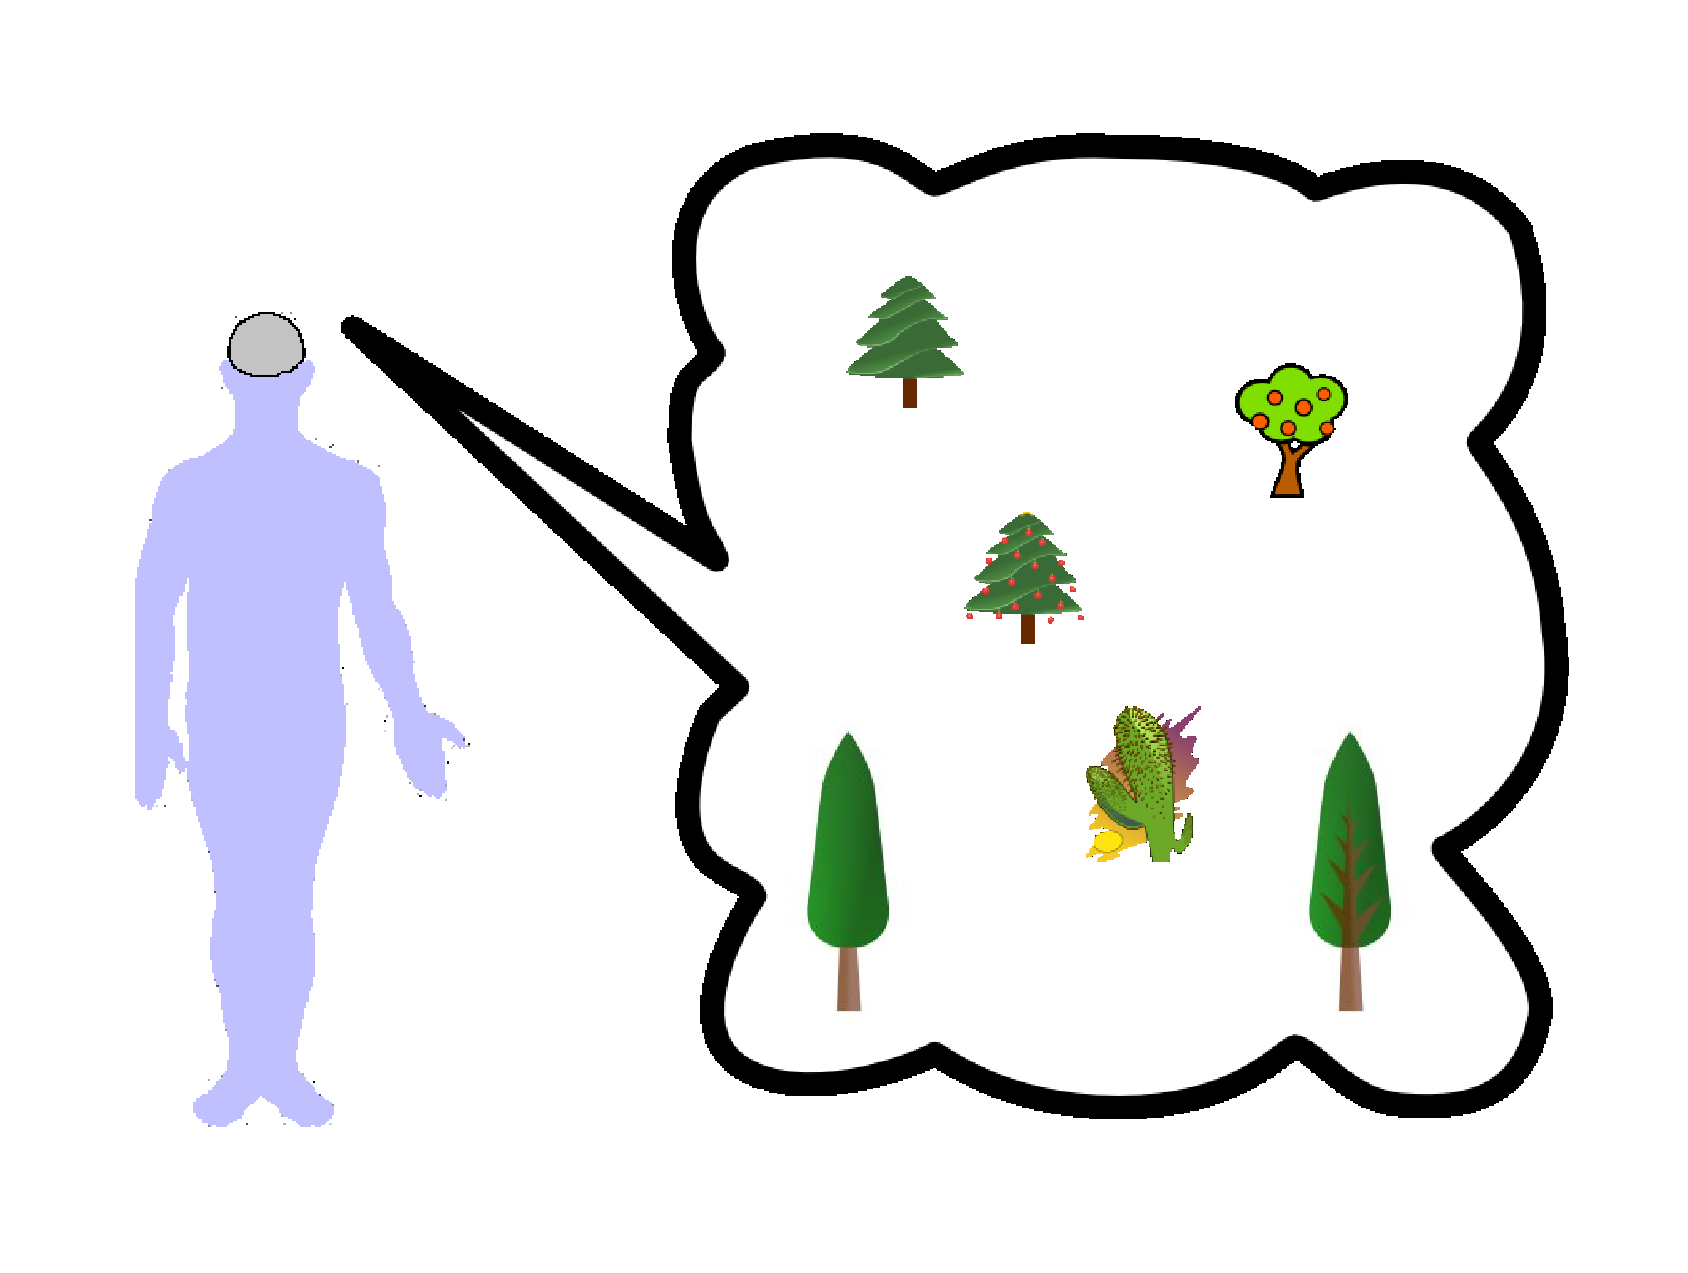
\includegraphics[scale=0.2]{vector/garden.eps}
        \caption{Data Garden}
        \label{garden_figure}
    \end{center}
\end{figure}

The interpreter (section \ref{cyboi_heading}) created in the work described in
this article stores all its knowledge in \emph{one single} tree, whose root
node it references. The single concepts (data bushes) are represented by
branches of that knowledge tree.

